\section{Teoría de Juegos}

La teoría de juegos es una herramienta fundamental para entender las estrategias en interacciones de todo tipo en la economía. Modelar sirve para entender los elementos que entran en juego los cuales se pueden instrumentalizar con tal de obtener una situación deseado, como puede ser incentivar la cooperación o la competencia en un mercado. 

Esta rama es fundamentalmente matemática, puede ser tan simple como compleja. En este capítulo se tratará lo más básico de teoría de juegos simultáneos, secuenciales, iterados y demás. 

La sustancia de un juego se compone de tres elementos: jugadores, estrategias y pagos. Los jugadores son quienes toman decisiones de manera estratégica para maximizar el pago posible que obtengan al final de un juego. El componente estratégico surge del hecho de que las decisiones de otros influyen los pagos que obtenga un jugador dada la decisión que tomó. En la economía hay multitud de estas interacciones, por ejemplo el precio fijado por una empresa afecta la demanda del bien de su competencia. 

Para introducirnos en la materia empezaron dando ejemplos (no necesariamente económicos) para definir juegos simultáneos.

\subsection{Juegos simultáneos}

En juegos simultáneos los jugadores toman decisiones al mismo tiempo, estas decisiones interactuan resultando en pagos. El pago a cada persona refleja un nivel de utilidad, por lo que cada agente buscará llegar a un resultado del juego (la combinación de acciones) que maximize su pago. 

Para dos agentes $A$ y $B$ cada uno toma la decisión $X$ o $Y$, la combinación de decisiones llevará a cierto nivel de pagos. Este escenario puede ser representado por una \textbf{matriz de pago}\marginnote{\textbf{Matriz de pago:} La matriz de pago es la representación de los pagos un juego dados ciertos jugaroes y estrategias posibles.}[-3cm] en el cuadro \ref{cuadro: matriz de pago genérica}.

\begin{table}[!htbp]
  
  \centering
  \caption{Matriz de pagos}
  \setlength{\extrarowheight}{2pt}
  \label{cuadro: matriz de pago genérica}
  \begin{tabular}{*{4}{c|}}
    \multicolumn{2}{c}{} & \multicolumn{2}{c}{$B$}\\\cline{3-4}
    \multicolumn{1}{c}{} &  & X  & Y \\\cline{2-4}
    \multirow{2}*{$A$}  & X & $(a,b)$ & $(c,d)$ \\\cline{2-4}
    & Y & $(e,f)$ & $(g,h)$ \\\cline{2-4} 
  \end{tabular}
\end{table}

La tabla nos dice que si $A$ tomó la estrategia $X$ y $B$ toma la decisión $Y$ entonces los pagos correspondientes son $(c,d)$, donde $c$ es el pago para $A$ y $d$ el pago para $B$. De la misma manera si $A$ elije $Y$ y $B$ decide $Y$ la matriz de pagos será $(g,h)$. 

La matriz también representa el componente estratégico mencionado en un inicio. Los pagos posibles para $A$ claramente dependen de las decisiones que tome $B$. Para poder decidir de manera estratégica los jugadores miran al futuro, si $A$ sabe que $B$ decide $X$ entonces $A$ elegirá la estrategia que maximize sus pagos. Específicamente $A$ está decidiendo con respecto a los pagos en negrita en el cuadro \ref{cuadro: B decide X}.

\begin{table}[!htbp]
  \centering
  \caption{Matriz de pagos con $B$ decidiendo $X$} \label{cuadro: B decide X}
  \setlength{\extrarowheight}{2pt}
  \begin{tabular}{*{4}{c|}}
    \multicolumn{2}{c}{} & \multicolumn{2}{c}{$B$}\\\cline{3-4}
    \multicolumn{1}{c}{} &  & X  & Y \\\cline{2-4}
    \multirow{2}*{$A$}  & X & $(\textbf{a,b})$ & $(c,d)$ \\\cline{2-4}
    & Y & $(\textbf{e,f})$ & $(g,h)$ \\\cline{2-4}  
  \end{tabular}
\end{table}

La decisión que tome $A$ dependerá qué pago es mayor, $a$ ó $e$, si es $a$ entonces elije $X$ y caso contrario elije $Y$.

Ahora veremos diversos juegos canónicos con el objetivo de aprender a resolver estos juegos y dar un análisis bajo criterio de Pareto de los mismos.

\subsection{El Dilema del Prisionero, un Juego Canónico}

El dilema del prisionero describe la situación en que dos criminales sospechosos son detenidos y separados para un proceso de interrogación. Si uno de los dos delata al otro y su complice no, este último tendrá pena de cárcel y el delator quedará libre. En caso de que los dos se delaten entre sí, ambos son condenados a años de cárcel. Por útlimo si ninguna se delata entre sí, quedan libres o cumplen penas menores.

La situación se ve reflejada en la matriz de pago del cuadro \ref{Juego: Prisionero}. Vemos que a mayor pena menores son los pagos. La solución de este juego es la siguiente.

\begin{table}[!htbp]
    \centering
    \caption{El dilema del prisionero}
    \setlength{\extrarowheight}{2pt}
    \begin{tabular}{*{4}{c|}}
      \multicolumn{2}{c}{} & \multicolumn{2}{c}{Prisionero $B$}\\\cline{3-4}
      \multicolumn{1}{c}{} &  & Cooperar  & Delatar \\\cline{2-4}
      \multirow{2}*{Prisionero $A$}  & Cooperar & $(-2,-2)$ & $(-10,-1)$ \\\cline{2-4}
      & Delatar & $(-1,-10)$ & $(-6,-6)$ \\\cline{2-4}
    \end{tabular} \label{Juego: Prisionero}
  \end{table}

Los jugadores deciden su estrategia óptima mirando hacia el futuro y prediciendo si es posible la decisión del otro. Si el prisionero $A$ piensa que $B$ lo delatará su respuesta óptima sería delatarlo también, dado que es la opción que minimiza sus años de cárcel. En caso de que $B$ coopere la respuesta óptima de $A$ sería delatar igualmente, dado que sigue siendo la opción que minimiza sus años de cárcel. Notemos que $A$ sigue la estrategia delatar independiente de la decisión de $B$, a esto se le llama una \textbf{estrategia dominante}\marginnote{\textbf{Estrategia Dominante:} }[0cm].

La matriz de pago es simétrica para ambos jugadores entonces llegamos a que $B$ sigue el mismo razonamiento por lo que delatar será también su estrategia dominante.

Dado que ambos tienen un estrategia dominante por delatar el resultado del juego será (Delatar, Delatar), dando un matríz de pago ($-6,-6$). Este punto se le conoce como \textbf{equilibrio de Nash}\marginnote{\textbf{Equilibrio de Nash:} }[0cm], es un punto tal que dada las decisiones tomadas por los demás jugadores ningun jugador tendrá incentivo a cambiar de decisión. Lo cual es equivalente a que cada uno eligió su estrategia óptima frente a las decisiones de los demás. En este caso sería que, dado que $B$ delató, $A$ no tiene incentivos a cambiar su decisión a cooperar, lo mismo se puede decir de $B$.

Hasta ahora hemos descrito un juego, es decir, jugadores, estrategias y pagos. Se resolvió este juego en específico donde dado que ambos jugadores tenían una estrategia dominante por delatar se llegó a un equilibrio de Nash. El siguiente paso es comentar sobre distintos aspectos del resultado bajo el criterio de Pareto.

El resultado fue (Delatar, Delatar) sin embargo otra posibilidad es que los jugadores hayan cooperado (Cooperar, Cooperar), en cuyo caso ambos jugadores están mejor. Esto bajo el criterio de Pareto se le llamaría una mejoría de pareto: si es que ambos cooperaran todos estarían mejor. Bajo esta perspectiva podemos decir que el equilibrio encontrado en este juego es sub-óptimo en términos de Pareto dado que hay un resultado posible mejor para ambos.

Este resultado es crucial pues es aplicable a un diversas situaciones económicas y políticas típicas, donde la cooperación nos llevaría a mejores resultados pero dada la desconfianza llegamos a un equilibrio sub óptimo. Por ejemplo, dos países con armas nucleares pueden acordar desarmarse para aumentar la seguridad mutua. Si ambos cumplen el acuerdo (cooperan), ambos estarán seguros y reducirán costos militares. Si uno cumple y el otro no (no coopera), el que deserta obtiene ventaja militar. Si ambos desertan y no desarman, continúan con altos costos y riesgos de conflicto. 

La gran moraleja económica en este caso es que dejar que los agentes decidan bajo sus propios intereses no siempre lleva al mejor resultado posible, la intervención en estos casos puede ser justificable. Ahora veremos otros juegos canónicos para describir otro tipo de situaciones.

\subsection{Otros Juegos Canónicos}

\textsc{Mano Invisible}

La matriz que representa este juego se encuentra en el cuadro \ref{Juegos: Mano}. La mano invisible describe cómo los individuos que buscan su propio beneficio personal, sin intención de hacerlo, contribuyen al bienestar general de la sociedad. Si se deja la autorregulación de los mercados, dado que los individuos persiguen su propio interés, se produce un equilibrio óptimo de Pareto. El agente $A$ tendrá una estrategía dominante la cual será la opuesta que el jugador $B$. Finalmente el equilibrio de Nash es eficiente paretianamente.

\begin{table}[!htbp]
    \centering
    \caption{La mano invisible}
    \setlength{\extrarowheight}{2pt}
    \begin{tabular}{*{4}{c|}}
      \multicolumn{2}{c}{} & \multicolumn{2}{c}{Agente $B$}\\\cline{3-4}
      \multicolumn{1}{c}{} &  & $X$  & $Y$ \\\cline{2-4}
      \multirow{2}*{Agente $A$}  & $X$ & $(0,10)$ & $(1,1)$ \\\cline{2-4}
      & $Y$ & $(11,11)$ & $(10,0)$ \\\cline{2-4}
    \end{tabular} \label{Juegos: Mano}
  \end{table}

%(Aquí se podría citar a Adam Smith)

\textsc{Guerra de los sexos}

Este juego se puede representar con la matriz del cuadro \ref{Juegos: Guerra}. La historia detras refiere a una pareja que se encuentra incomunicada en medio de un festival de música. Ambos tienen gustos diferentes, al hombre le gusta el Reggae mientras que a la mujer le gusta el EDM. Dado que están separados e incomunicados quieren encontrarse, pero también quieren ir al concierto que sea la música de su gusto. Es por eso que reciben utilidad tanto de encontrarse como de ir al concierto que les gusta, maximizan su utilidad si es que van al concierto de su preferencia y encuentran a su pareja ahí.
\begin{table}[!htbp]
    \centering
    \caption{Guerra de los sexos}
    \setlength{\extrarowheight}{2pt}
    \begin{tabular}{*{4}{c|}}
      \multicolumn{2}{c}{} & \multicolumn{2}{c}{Mujer}\\\cline{3-4}
      \multicolumn{1}{c}{} &  & Reggae  & EDM \\\cline{2-4}
      \multirow{2}*{Hombre}  & Reggae & $(2,1)$ & $(1,1)$ \\\cline{2-4}
      & EDM & $(0,0)$ & $(1,2)$ \\\cline{2-4}
    \end{tabular} \label{Juegos: Guerra}
  \end{table}

En este juego canónico cada uno tiene estragia dominante por ir al concierto de su banda preferida independiente de lo que haga el otro. Por tanto hay dos equilibrios de Nash, para resolver este juego habría que incluir estrategias mixtas lo cual veremos proximamente.

\textsc{La caza del venado}

La matriz de este juego se encuentra en el cuadro \ref{Juegos: Venado}. Dos individuos van a cazar ya sea conejos o venados y deben escoger su presa sin conocer la elección del otro cazador. Para cazar el venado (un premio mayor) requieren de la ayuda del otro, mientras que un conejo puede ser cazado sin ayuda de otro. Por lo tanto, si cooperan cazando al venado podrán ambos obtener más beneficios y estár en un óptimo de Pareto.

\begin{table}[!htbp]
    \centering
    \caption{La caza del venado}
    \setlength{\extrarowheight}{2pt}
    \begin{tabular}{*{4}{c|}}
      \multicolumn{2}{c}{} & \multicolumn{2}{c}{Cazador $B$}\\\cline{3-4}
      \multicolumn{1}{c}{} &  & Venado  & Conejo \\\cline{2-4}
      \multirow{2}*{Cazador $A$}  & Venado & $(4,4)$ & $(0,3)$ \\\cline{2-4}
      & Conejo & $(3,0)$ & $(3,3)$ \\\cline{2-4}
    \end{tabular} \label{Juegos: Venado}
  \end{table}
En este caso no existen estrategias dominantes, lo que lleva a la existencia de dos equilibrios de Nash, cazar al venado juntos domina paretianamente a cazar conejos juntos. Lo anterior representa un problema de cooperación social y una dicotomía entre seguridad y cooperación. 

\textsc{Chicken}. 

La matriz de este juego se encuentra en el cuadro \ref{Juegos Chicken}. Se trata de un juego para determinar quien es el más valiente, dos personas se posicionan con sus autos en dos extremos y aceleran de manera que llegará un punto en que choquen entre si. El primero que doble para evitar el impacto es un gallina, dejando al ganador como valiente. Hay tres escenarios, el primero en que uno de los dos dobla y queda como gallina, un segundo escenario en donde los dos doblan ambos quedando como gallinas y por último el caso en que chocan. 

Ambos corredores quieren hacer lo opuesto a lo que haga el otro, los equilibrios de Nash serían entonces los que uno de ellos dobla y el otro sigue.\footnote{Rising, L: The Patterns Handbook: Techniques, Strategies, and Applications, page 169. Cambridge University Press, 1998. \textbf{Schedule Chicken}.}
\begin{table}[!htbp]
    \centering 
    \caption{Chicken}
    \setlength{\extrarowheight}{2pt}
    \begin{tabular}{*{4}{c|}}
      \multicolumn{2}{c}{} & \multicolumn{2}{c}{Corredor $B$}\\\cline{3-4}
      \multicolumn{1}{c}{} &  & Ceder (gallina)  & Seguir (valiente) \\\cline{2-4}
      \multirow{2}*{Corredor $A$}  & Ceder (gallina) & $(2,2)$ & $(1,3)$ \\\cline{2-4}
      & Seguir (valiente) & $(3,1)$ & $(0,0)$ \\\cline{2-4}
    \end{tabular} \label{Juegos Chicken}
  \end{table}

\subsection{Juegos secuenciales}

Los juegos secuenciales son una forma extendida de los juegos simultáneos. Bajo juegos simultáneos las estrategias eran acciones individuales; confesar, delatar, cooperar, tracionar, etcéra, bajo juegos secuenciales las estrategias son un grupo de acciones en determinado orden. 

Los juegos secuenciales tienen un orden cronológico de la toma de decisiones y se juega por turnos. Para representar esto tendremos que usar ramas (figura \ref{Secuencia Soviética}), la decisión de un jugador abre las posibles decisiones del otro jugador que llevará a otra rama de decisiones con las que podrá responder el jugador inicial.

Un ejemplo que nos podrá servir sería el dominio de Berlin en la guerra fría. En un caso en donde la Unión Soviética (URSS) pide que las potencias occidentales abandonen Berlín, en cuyo caso Estados Unidos (EEUU) puede aceptar o no aceptar la orden. En caso de aceptar EEUU pierde -5 en pagos y la URSS gana 10. En caso de no aceptar el juego no termina ahí, se abre la posibilidad de que la URSS responda bélicamente o que simplemente los bloquee (figura \ref{Secuencia Soviética}). 
\begin{figure}[htb]
  \centering
  \caption{Juego Secuencial del dominio sobre Berlín}
  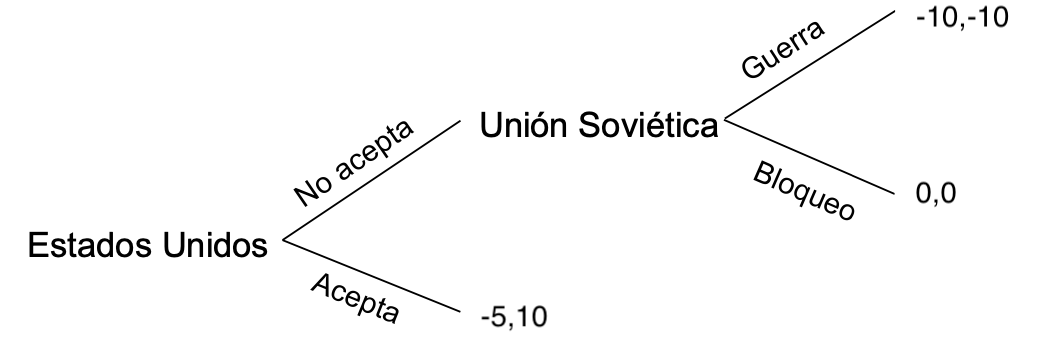
\includegraphics[width=10cm]{Figuras/juegos secuencia.png}
  \label{Secuencia Soviética}
\end{figure}
% falta hacerla en el formato.

Las estrategias serán más de una decisión, en esta caso serían (Acepta, No Acepta y Guerra, No Acepta y Bloqueo).

Para resolver estos juegos uno tiene que seguir un método inductivo, resolver desde el futuro hacia el pasado. De esta manera los jugadores pueden distinguir de las amenazas creíbles y no creíbles. Por ejemplo, la respuesta bélica de la URSS no es una amenza creíble puesto que esta queda mejor simplemente bloquando a EEUU. Por lo tanto EEUU sabe que la URSS responderá con bloqueo, entonces la estrategia de EEUU se reduce a no aceptar la orden puesto que obtendra un pago mayor ($0$) al caso en donde acepta abandonar Berlín ($-5$).

En resumen los juegos secuenciales tienen que resolverse desde el futuro al pasado para distinguir amenazas creíbles. Plantear este juego como si fuera simultáneo nos llevaria a considerar un equilibrio de Nash que no es secuencialmente racional (cuadro \ref{simult Berlín}). Bajo esa matriz de pago el aceptar es un equilibrio de Nash, pero planteándolo secuencialmente podremos notar EEUU solo aceptará en caso de que la respuesta bélico de la URSS sea creíble (en este caso no lo es).

\begin{table}[!htbp]
    \centering
    \caption{Dominio sobre Berlín}
    \setlength{\extrarowheight}{2pt}
    \begin{tabular}{*{4}{c|}}
      \multicolumn{2}{c}{} & \multicolumn{2}{c}{Unión Soviética}\\\cline{3-4}
      \multicolumn{1}{c}{} &  & Guerra & Bloqueo \\\cline{2-4}
      \multirow{2}*{Estados Unidos}  & Acepta & $(\underbar{-5},\underbar{10})$ & $(-5,10)$ \\\cline{2-4}
      & No acepta & $(-10,-10)$ & $(\underbar{0},\underbar{0})$ \\\cline{2-4}
    \end{tabular} \label{simult Berlín}
  \end{table}

Resolver un juego secuencial por el método inductivo nos llevará a encontrar un equilibrio perfecto en subjuegos. 

\begin{figure}[htb]
  \centering
  \caption{Solución del Juego Secuencial de Berlín}
  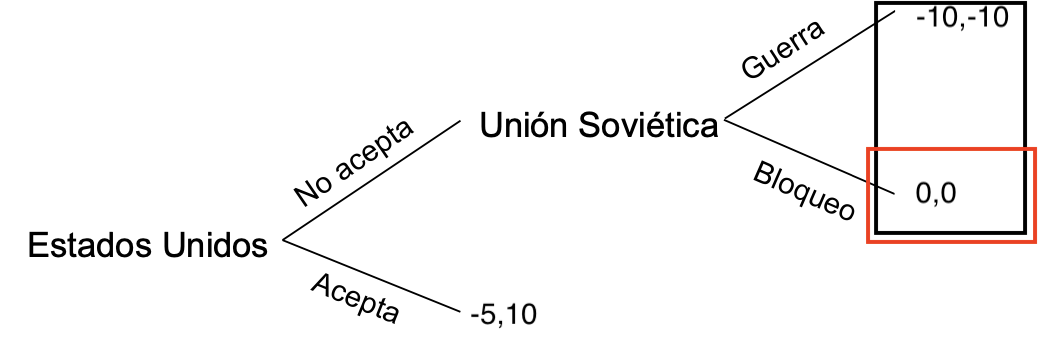
\includegraphics[width=10cm]{Figuras/Inducción.png}
  \label{Solución Soviética}
\end{figure}

¿Cuál es la relación entre Equilibrio de Nash (EN) y Equilibrio Cerfecto en Subjuegos (EPS)? En un juego secuencial puedes obtener EN que no sean coherentes con las amenazas creíbles. Los EPS siempre son coherentes con la credibilidad de las amenazas. En este sentido un EN no siempre es un EPS, pero un EPS siempre es un EN.

\subsection{Estrategias Mixtas}

Hasta ahora hemos vistos diversos juegos que no tienen un resultado certero, por ejemplo en \textit{Chicken} ambos jugadores buscan hacer lo opuesto al otro. Por lo que el salir perdiendo o ganando se reduce a tratar de sorprender al otro, por lo que la incertidumbre es un elemento fundamental de este tipo de intereacciones.  

La incertidumbre únicamente algo con lo que lidiar sino que puede ser instrumentalizada: las auditorias aleatorias con tal de fiscalizar tienen el objetivo de disuadir comportamientos fuera de regla. En este sentido el jugador fiscalizador no elige una pura estrategia como podría ser fiscalizar siempre, lo cual sería altamente costoso. En este caso conviene asignar probabilidades a cada estrategia (fiscalizar, no fiscalizar), con tal de disuadir comportamientos fuera de regla mientras se minimizan costos.

Lo que vamos a hacer será cambiar las reglas del juego: Anteriormente teníamos estrategias puras, los jugadores tenían que decidir la acción que tomar, ahora les pediremos a los jugadores que eligan un vector de probabilidades que le deben de asignar a cada decisión. Esta re estruturación del juego nos permitirá tener una idea más clara del resultado en juegos donde habían más de un equilibrio de Nash. Las estrategias mixtas entonces consisten en asignar una probabilidad entre 0 y 1 a cada una de las posibles estrategias disponibles con tal de que todas sumen 1. Tomemos el juego sencillo y asignemosle una probabilidad a cada estrategia. En los penales del Futbol la idea es predecir que lado elegirá el contrario para patear al otro lado o atajar a ese mismo lado. Bajo este contexto podemos definir la siguiente matriz de pago. 
\begin{center}
\begin{tabular}{*{4}{c|}}
  \multicolumn{2}{c}{} & \multicolumn{2}{c}{Arquero}\\\cline{3-4}
  \multicolumn{1}{c}{} &  & Izquierda & Derecha \\\cline{2-4}
  \multirow{2}*{Jugador}  & Izquierda & $(0,0)$ & $(1,-1)$ \\\cline{2-4}
  & Derecha & $(1,-1)$ & $(0,0)$ \\\cline{2-4}
\end{tabular} 
\end{center}

Por lo tanto cada jugador asignará una probabilida  $p$ o $q$ a tirar a la derecha y por descarte (la suma de las probabilidades deben ser uno) la otra estrategia se tomará con una probabilidad $1-p$ y $1-q$.

\begin{center}
\begin{tabular}{cccc}
  Estrategias & Probabilidad & Pago Jugador & Pago Arquero \\
  D,D & $p\cdot q$ & 0 & 0 \\
  D,I & $p \cdot (1-q)$ & 1 & -1 \\
  I,D & $(1-p)\cdot q$ & 1 & -1 \\
  I,I & $(1-p)\cdot (1-q)$ & 0 & 0 
\end{tabular}
\end{center}

Por lo tanto la esperanza de pagos (utilidad) en este caso será para cada uno,
\begin{align*}
  \mathbb{E}(U^J) =& pq\cdot 0 + p(1-q)\cdot 1 + (1-p)q\cdot 1 + (1-p)(1-q)\cdot 0 + p \\
  = & p-qp + q-pq = p(1-2q) + q
\end{align*}
El caso del arquero tendrá la siguiente utilidad esperada,
\begin{align*}
  \mathbb{E}(U^A) =& pq \cdot 0 + p(1-q)\cdot(-1) + (1-p)q \cdot (-1) + (1-p)(1-q) \cdot 0 \\ = & -p+pq -q+pq = q(2p-1)-p
\end{align*}
Lo que necesitamos para encontrar el equilibrio de Nash es entender la función de reacción óptima, en el caso del jugador que patea este debe decidir $p$ en función de $q$. En la utilidad esperada del jugador la parte importante de analizar será el término $(1-2q)$ lo demás lo podemos tomar como constante. En específico nos preguntaremos que hacer en caso de que $1-2q$ sea mayor, igual o menor a cero.
\begin{itemize}
  \item En caso de que $q > 1/2$ entonces el arquero tiene una mayor probabilidad de tirarse a la derecha, por lo que la función de reacción óptima indicaría que habría que patear a la izquierda. Fíjese que si $q>1/2$ entonces $1-2q<0$ por lo que para maximizar la utilidad esperada habría que asignar $p = 0$. Básicamente, si es más probable que el arquero se tire a la izquierdo entonces asigno $100\%$ de proabilidad de patear hacia la izquierda. 
  \item El caso contrario en que el arquero tenga una mayor probabilidad de tirarse a la izquierda $q<1/2$ el jugador maximizará su utilidad esperada pateando a la derecha. Para tal $q$ el término $1-2q>0$ por lo que conviene aumentar la probabilidad de patear a la derecha al máximo. 
  \item Por último en caso de que $q = 1/2$ no hay una probabilidad óptima certera entonces se toma un $p$ cualquiera entre 0 y 1.\footnote{Técnicamente esta respuesta no es una función pues asigna más de resultado a un solo punto del dominio. Para efectos del curso esto no genera ningún problema.}
\end{itemize}
